\newpage
\section{Implementacja na platformie Google Cardboard}
\paragraph{}
Innym przykładem implementacji projektu w rozszerzonej rzeczywistości może być platforma Google Cardboard \footnote{https://vr.google.com/cardboard/index.html}. Są to niskobudżetowe okulary stworzone przez firmę Google do wyświetlania wirtualnej rzeczywistości. Kartonowe okulary powstawły w celu wyświetlania obrazu stereoskopowego. Posiadają one miejsce do umieszczenia dowolnego telefonu komórkowego typu smartphone. Do projektu wybrano wersję, która pozwala na umieszczenie telefonu w sposób taki, iż tylna kamera nie jest załonięta przez obudowę. Dzięki temu można użyć platformę Cardboard przeznaczoną pierwotnie tylko do wirtualnej rzeczywistości do stworzenia aplikacji wykorzystującą augmented reality.

\begin{center}
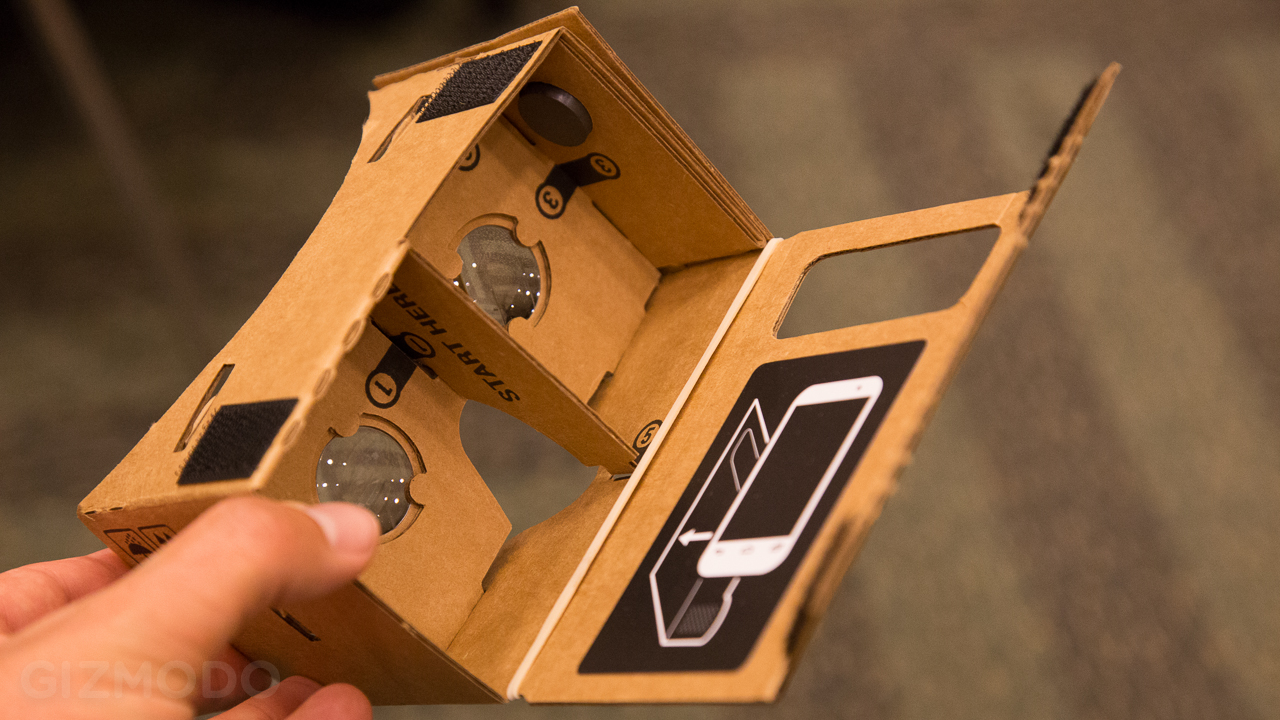
\includegraphics[width=0.9\textwidth]{images/cardboard.jpg}
\captionof{figure}{
Google Cardboard w wersji do samodzielnego złożenia
}
\small {źródło: http://gizmodo.com/turn-your-android-into-a-virtual-reality-headset-with-g-1596026538 }
\end{center}

\paragraph{}
Dzięki użyciu kamery użytkownik widzi obraz znajdujący się przed nim. Aby obraz był stereoskopowy należało stworzyć aplikację, która wyświetlić strumień danych z kamery dzieląc go na dwa obrazy (kolejno dla lewego oraz prawego oka).

\begin{center}
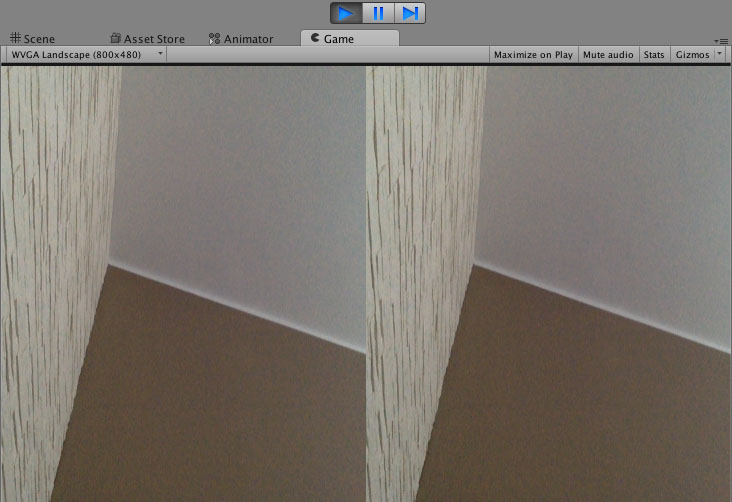
\includegraphics[width=0.9\textwidth]{images/kadr.jpg}
\captionof{figure}{
Ujęcie z kamery aparatu w obrazie stereoskopowym - scena w Unity
}
\small {źródło własne}
\end{center}

\subsection{ArToolkit}
\paragraph{}
W celu wyświetlenia wirtualnych obiektów na obrazie z kamery rozbudowano aplikację z rodziału pierwszego {\color{red}uzupełić rozdział}. Do platformy Unity doinstalowano zewnętrzny komponent ARToolKit  \footnote{http://artoolkit.org/}. Jest to biblioteka wydana przez University of Washington \footnote{https://www.hitl.washington.edu/artoolkit/}, lecz obecnie upostępniona jest na licencji GNU. Kod źródłowy jest otwarty i rozwijany przez środowisko Open Source \footnote{https://github.com/artoolkit}.
\subsection{Markery}
\paragraph{}
Za pomocą tej biblioteki możliwe jest wykrywanie w obrazie z kamery markerów, czyli specjalnie przygotowanych czarno-białych obrazków (w naiwnej implementacji - wydrukowanych na kartkach), oraz nakładanie w ich miejsce trójwymiarowych modeli lub całych scen. Dzięki bibliotece ArToolkit możliwe jest diagnozowanie pod jakim kątem padania oraz w jakiej odległości od urządzenia znajduje się marker. Umiejscowienie tagu analizowane jest w czasie rzeczywistym, co zapewni ciągłą korekcję ułożenia wirtualnych modeli względem ich realnych odpowiedników.

\begin{center}
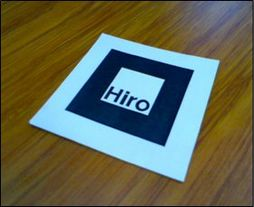
\includegraphics[width=0.9\textwidth]{images/hiro.png}
\captionof{figure}{
Przykład przygotowanego obrazka do rozpoznawania - marker
}

\end{center}
\paragraph{}
Szablony markerów można wykonywać we własnym zakresie. Aby zaimportować nowe obrazki do biblioteki ArToolkit należy przygotować specjalny plik binarny reprezentujący model markera.
\footnote{http://bit.ly/1YU199f}.

\begin{center}
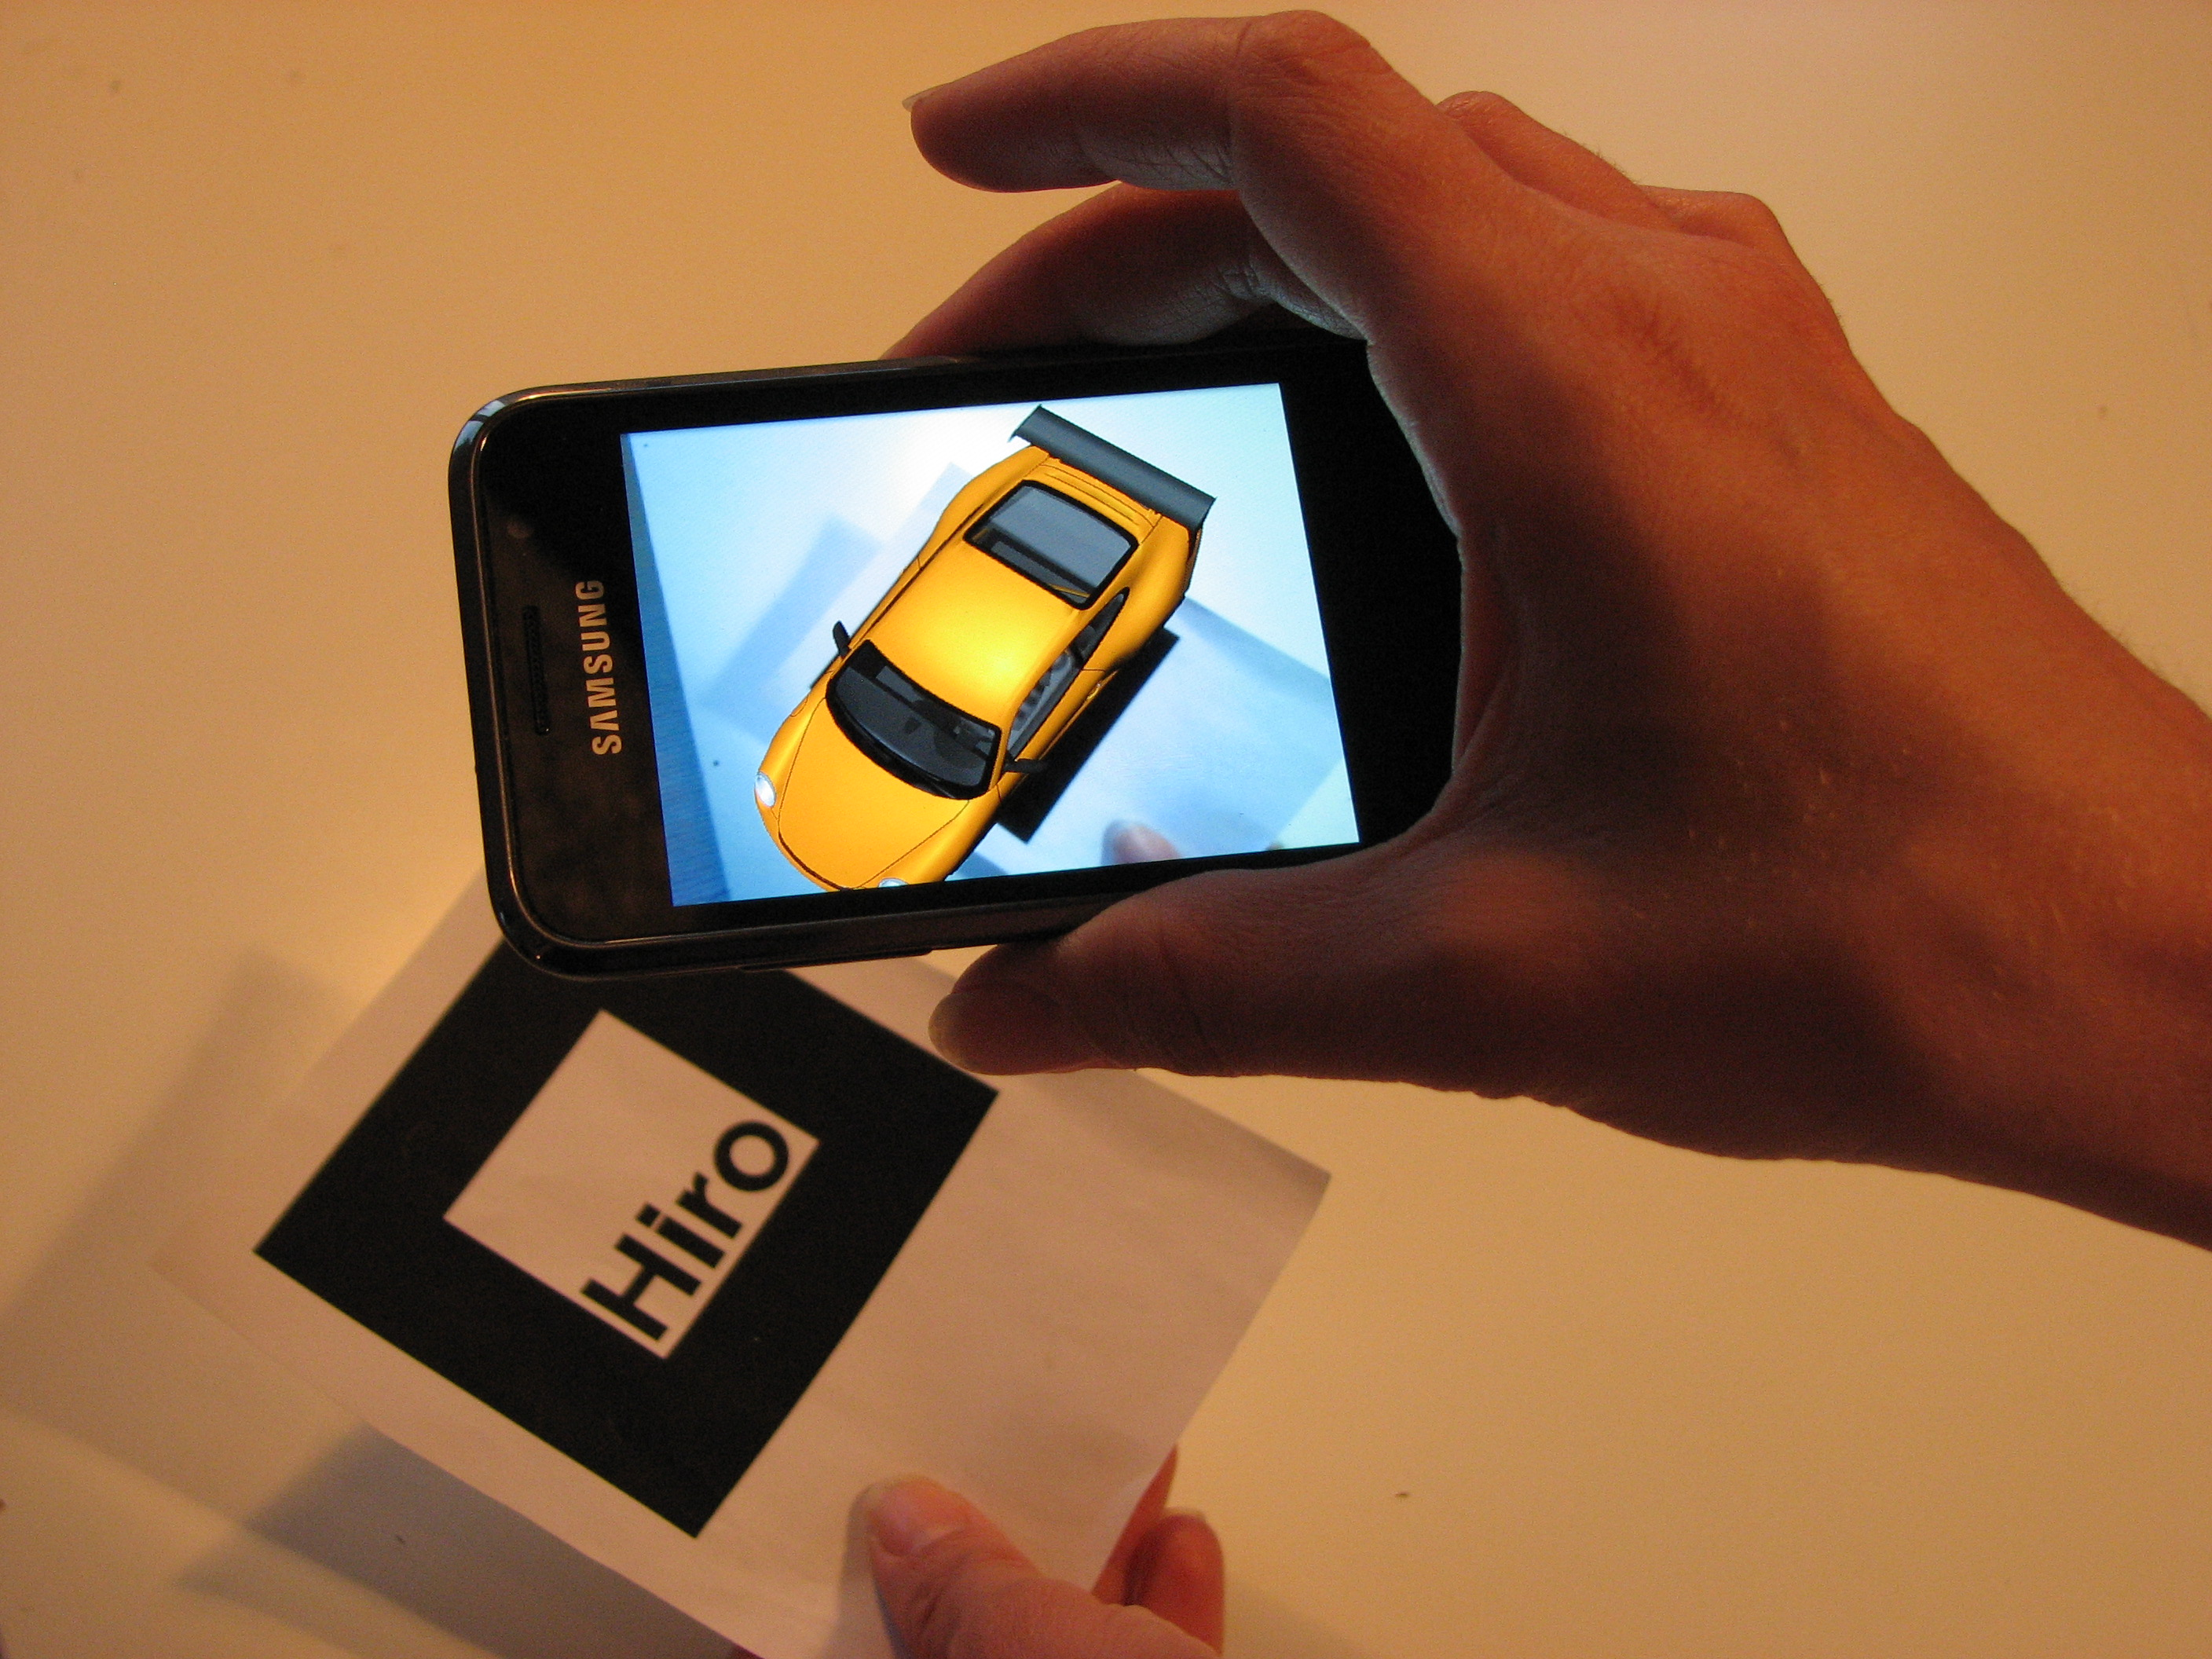
\includegraphics[width=0.9\textwidth]{images/artoolkit-demo.jpg}
\captionof{figure}{
Przykład zastosowania markera w ARToolkit
}
\small {źródło http://arblog.inglobetechnologies.com/?p=421}
\end{center}
\subsection{Przykład implementacji}
\paragraph{}
{\color{red}Opisać}
\begin{center}
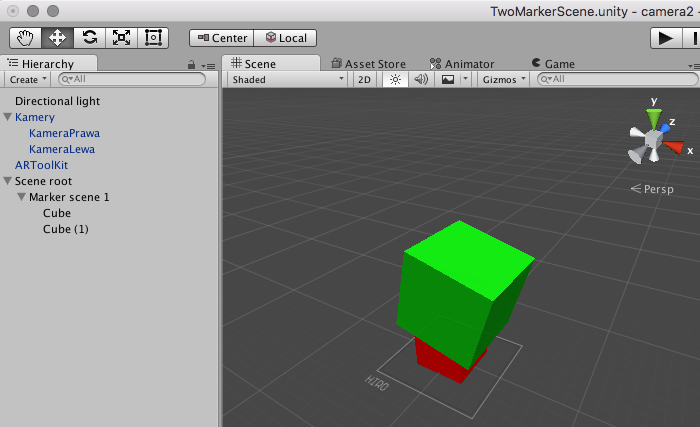
\includegraphics[width=0.9\textwidth]{images/artoolkit-przyklad.png}
\captionof{figure}{
Podstawowa impementacja
}
\small {źródło własne}
\end{center}
\subsection{Napotkane problemy i ograniczenia}
\paragraph{}
\begin{enumerate}
	\item Proces renderowania musi odbywać się na telefonie komórkowym, gdyż obraz kamery jest ciągle analizowany. Przy dużych scenach stworzonych w Unity moc obliczeniowa urządzenia jest niewystarczająca.
	\item Analizowanie pozycji markera przy nieustannie włączonej kamerze powoduje dużą drenację baterii urządzenia. Czas pracy na baterii jest mocno ograniczony
	\item Unity w wersji Personal (darmowej) skompilowanej pod platrformę mobilną (np. Android) nie udostępnia obsługi sieci (np. za pomocą połączenia TCP). Nie pozwala to na połączenie z zenętrznym kontrolerem.
	\item Sterowanie za pomocą kontrolera bez fizycznych przycisków z założonymi okularami Google Cardboard jest bardzo uciążliwe. W przyszłości należałoby rozważyć połączenie telefou z zewnętrznym kontrolerem typu PAD\footnote{https://pl.wikipedia.org/wiki/Gamepad}.
\end{enumerate}

\paragraph{}
{\color{red}a moze dopisać porownanie z gearvr?}